\documentclass[preprint,12pt]{elsarticle}

\usepackage{amssymb}
\usepackage{color}
\usepackage{graphicx}
\usepackage{placeins}
\usepackage{cleveref}
\usepackage[margin=2.5cm]{geometry}
\usepackage{appendix}
\usepackage{gensymb}

\usepackage{lineno}

\journal{Journal of Nuclear Materials}

\begin{document}

\begin{frontmatter}



\title{An \textit{ab initio} molecular dynamics study of varied compositions of the LiF-NaF-KF molten salt}
\author[inst1]{Veronica Heyl}

\affiliation[inst1]{organization={North Carolina State University},%Department and Organization 
            city={Raleigh},
            postcode={27607}, 
            state={NC},
            country={USA}}

\author[inst1,inst2]{Benjamin Beeler}

\affiliation[inst2]{organization={Idaho National Laboratory},%Department and Organization
            city={Idaho Falls},
            postcode={83415}, 
            state={ID},
            country={USA}}

\begin{abstract}

With increasing interest in molten salt reactors, there becomes a demand for investigations into thermophysical properties of salt systems. The LiF-NaF-KF (FLiNaK) salt system is a primary candidate for use in these reactors. However, the thermophysical properties of compositions outside the eutectic composition are still largely unknown. In this article, properties of ten unique compositions, including four ternary compositions, are investigated using \textit{ab initio} molecular dynamics simulations across five temperatures between 900 K and 1300 K. The properties of interest are the density, thermal expansion, bulk modulus, compressibility, heat capacity, and enthalpy of mixing. In general, the results were found to be in good agreement with other literature and experimental results. The density and heat capacity had a tendency to be slightly underpredicted. No conclusions could be drawn about the bulk modulus and compressibility in terms of compositional dependence. The thermal expansion had a negative trend with respect to the LiF concentration and no trends were observed for the NaF or KF concentration. The enthalpy of mixing shows minima for the ternary compositions, with the near-equiatomic composition exhibiting the lowest values. This work shows the potential for compositional tailoring in the FLiNaK system to optimize thermophysical properties.

\end{abstract}



\begin{keyword}
%% keywords here, in the form: keyword \sep keyword
molten salts \sep thermophysical properties \sep AIMD \sep FLiNaK
\end{keyword}

\end{frontmatter}

\linenumbers


\section{Introduction}
\label{sec:sample1}


Molten salts are ionic liquid mixtures at high temperatures with high heat capacity and thermal conductivity. These properties make molten salts useful as a coolant or fuel salt for molten salt reactors (MSRs). Research into MSRs was largely neglected after the experiments by Oak Ridge National Laboratory during the late 1960s\cite{Porter2022}. The advantages of an MSR compared to solid fuel reactors are that MSRs do not need traditional fuel fabrication, possess increased intrinsic safety, and have a high working temperature\cite{MSROverview}. Because of their benefits, there has been renewed interest in MSRs in the past few years. With this comes the need to characterize molten salts and determine their thermophysical properties, which are required to parameterize complex fluid dynamics and chemical interaction models\cite{Porter2022,freile2019}.


The LiF-NaF-KF (FLiNaK) salt system is one of the primary candidates to operate as a coolant salt in MSRs. FLiNaK has been proposed as the heat transfer medium in the Very High-Temperature Reactor, a graphite-moderated, gas-cooled Generation IV concept reactor\cite{Benes2009}, and is of interest to serve as the primary coolant in MSRE-type designs. FLiNaK is also often utilized as a surrogate for LiF-BeF$_2$ (FLiBe), which is also of interest in MSRs, but more challenging to explore experimentally due to the toxicity of Be. The volumetric heat capacity for FLiNaK is similar to water but without the issue of critical heat flux due to the large margin to boiling. Additionally, FLiNaK can operate under ambient pressure conditions, allowing for the removal of the high system pressure in water-cooled reactors \cite{Ambrosek2009}. Thus, a significant amount of experimental research has been performed on FLiNaK to determine select thermophysical and chemical properties.  

Frandsen et al. investigated the density as a function of temperature between approximately 500\degree C and 1500\degree C, the total scattering structure function, and the pair distribution function of the eutectic composition\cite{Frandsen2020}. Anderson et al. collaborated with Oak Ridge National Laboratory to determine the density, equilibrium volume, coefficient of thermal expansion, self-diffusion coefficients for constituent ions at 973 K, 1223 K, and 1423 K, and the self-diffusion coefficient for solute ions at 973 K\cite{Anderson2015}. All of these properties were determined at the eutectic composition. Liu et al. studied the microstructures of lutetium fluoride and oxyfluoride structures in eutectic FLiNaK using Raman spectroscopy and density functional theory\cite{Xiyan2021}. Ambrosek et al. used previously acquired experimental data to determine the heat transfer of the eutectic composition in comparison to the Dittus-Boelter correlation\cite{Ambrosek2009}. Additional experiments have been performed on the eutectic composition \cite{Hoffman1955,Holcomb2010,Yoder2014}.

Thermophysical properties are difficult to determine experimentally because of the toxicity of salts, the targeted high temperatures, and the cost of the experiment \cite{Porter2022}. In lieu of an abundance of high-fidelity experimental data, a computational approach can be pursued to complement and supplement the existing experimental data. Salanne et al. constructed interatomic potentials for mixtures of LiF, NaK, KF, and ZrF$_4$ and used them for molecular dynamics simulations to evaluate the heat-transfer properties of FLiNaK and NaF-ZrF$_4$\cite{Salanne2009}. Lee et al. used molecular dynamics to train neutral network forcefields and reparametrized analytical forcefields in order to use large-scale molecular dynamics in the determination of structural and transport properties\cite{Lee2021}. Sona et al. used computational fluid dynamics simulations to investigate the flow and heat transfer characteristics of eutectic FLiNaK\cite{Sona2014}. Recently, \textit{ab initio} molecular dynamics simulations (AIMD) have begun to be explored to determine thermophysical properties, structure, and speciation in FLiNaK\cite{Nam2014,Frandsen2020,Clark2020,Sprouster2022}. 

The common trend among previous works is the selection of investigating only the eutectic composition. As most experimental work has been done on this composition, previous computational work purposely and appropriately chose to focus on the composition that had data available for comparison. While understandable, due to corrosion, changing redox potential, and other variables in a reactor environment, the composition of the salt may slightly change as a function of time. Additionally, while the eutectic composition has the minimum melting point for this ternary system, there may be other properties (density, viscosity, heat capacity, etc.) that are more beneficial at non-eutectic compositions, but which are largely unknown\cite{Benes2009}. While both thermophysical and transport properties are required for the correct implementation of molten salts in a reactor system, the initial evaluation of thermophysical properties, which are more easily obtainable through both experimental and computational efforts \cite{Duemmler2022,Duemmler2023,Zhao2023}, provides an initial step in the full property evaluation of key molten salt systems. Thus, only thermophysical properties are the focus of this manuscript. 

This work seeks to more fully characterize the thermophysical properties of FLiNaK through a first principles computational investigation of four ternary compositions (including the eutectic), three binary eutectic compositions, and three pure alkali-halide salt constituents. The density, bulk modulus, compressibility, heat capacity, thermal expansion, and enthalpy of mixing for each different composition in the FLiNaK system will be determined using appropriate temperatures between 900 K and 1300 K. This is the most extensive investigation of thermophysical properties across the compositional and temperature regimes in the nuclear-relevant molten salt FLiNaK.

\section{Computational Methods}
Ten unique compositions (all compositions are stated in mole percent) were studied for the LiF-NaF-KF salt system, including four ternary compositions (eutectic 46-12-42, 16-42-42, 32-34-34, and 42-42-16), three binary eutectic compositions (0-40-60, 51-0-49, and 61-39-0), and the three pure alkali-halide salt constituents (LiF, NaF, and KF). The initial structure was prepared by inserting the respective molecules into a supercell via the Packmol package \cite{Packmol}, with 100 atoms for the ternary systems and 200 atoms for all other systems. Such system sizes have been shown to produce converged and comparable results for AIMD analyses of molten salts \cite{Bengtson2013,Andersson2022}. AIMD simulations were performed using the Vienna \textit{ab initio} Simulation Package (VASP)\cite{VASP1,VASP2,VASP3}. The temperature range investigated for each composition depended upon the corresponding melting point of that composition, with the ternary system temperatures ranging from 900 K to 1300 K, binary system temperatures from 1000 K to 1300 K, and the pure constituent temperatures from 1100 K to 1300 K. The energy cutoff was 600 eV, which is 100 eV higher than the recommended maximum for the pseudopotentials utilized, and the electronic optimization criterion was 10\textsuperscript{-3} eV. Convergence testing was performed with more fine energy convergence criteria to ensure that the results were not affected by the choice of electronic optimization. A 1$\times$1$\times$1 k-point mesh was used, as this has been shown to be sufficient in prior simulations for molten salts with similarly sized supercells\cite{Duemmler2022,Nam2014}. The vdW-DF2 van der Waals functional was used to account for the dispersion interactions\cite{vdWDFT1,vdWDFT2}. While there are many choices of dispersion interactions available within VASP, this specific choice was made due to its ability to replicate the properties of various chloride salts\cite{Duemmler2022}. A brief examination of the DFT-D3 dispersion correction term \cite{grimme2010} was also explored, which did not show superior predictions.

In the Open Visualization Tool (OVITO)\cite{Ovito}, the initial structures were verified to have no bonds shorter than 1.5 \AA, indicating a reasonable initial guess. The structures were equilibrated using VASP at each temperature studied. The initial equilibrium simulation for each composition occurred at 1100 K. The energy was evaluated versus time to check if the system was equilibrated. If the slope of the running average was approximately zero, the structure was considered to be at equilibrium. If not, the simulation was continued until it was determined that equilibrium was reached. Typically, equilibration takes approximately 10-15 ps.

Utilizing the equilibrated structures, the system was further evolved at different specified volumes to obtain the pressure as a function of volume. The systems were equilibrated for a further 4 ps, with time-averaging to determine the energy and pressure over the final 3 ps. At least six data points were included for each composition and temperature, ensuring that the pressures ranged from -2 to +10 kbar, with at least one pressure greater than 5 kbar. This is in accordance with a prior procedure utilized\cite{Duemmler2022}. Five simulations were performed for each unique volume for statistical significance. Thus, for a given composition and temperature, approximately thirty simulations were performed. The pressure as a function of the volume, shown in \cref{fig:PV_PE}a, was determined by fitting a quadratic equation, allowing for the determination of the volume at which the pressure is zero. 

The zero pressure volume, along with the mass, was used to calculate the density. The parabolic fit of the volume-pressure curve was used to calculate the bulk modulus and compressibility:
\begin{equation}\label{eq:bulk}
K = -V\left(\frac{\partial{P}}{\partial{V}}\right)_{P=0}= \frac{1}{\beta}
\end{equation}
\noindent where K is the bulk modulus, V is the volume, P is the pressure, and $\beta$ is the compressibility. 

\begin{figure}[!h]
\centering
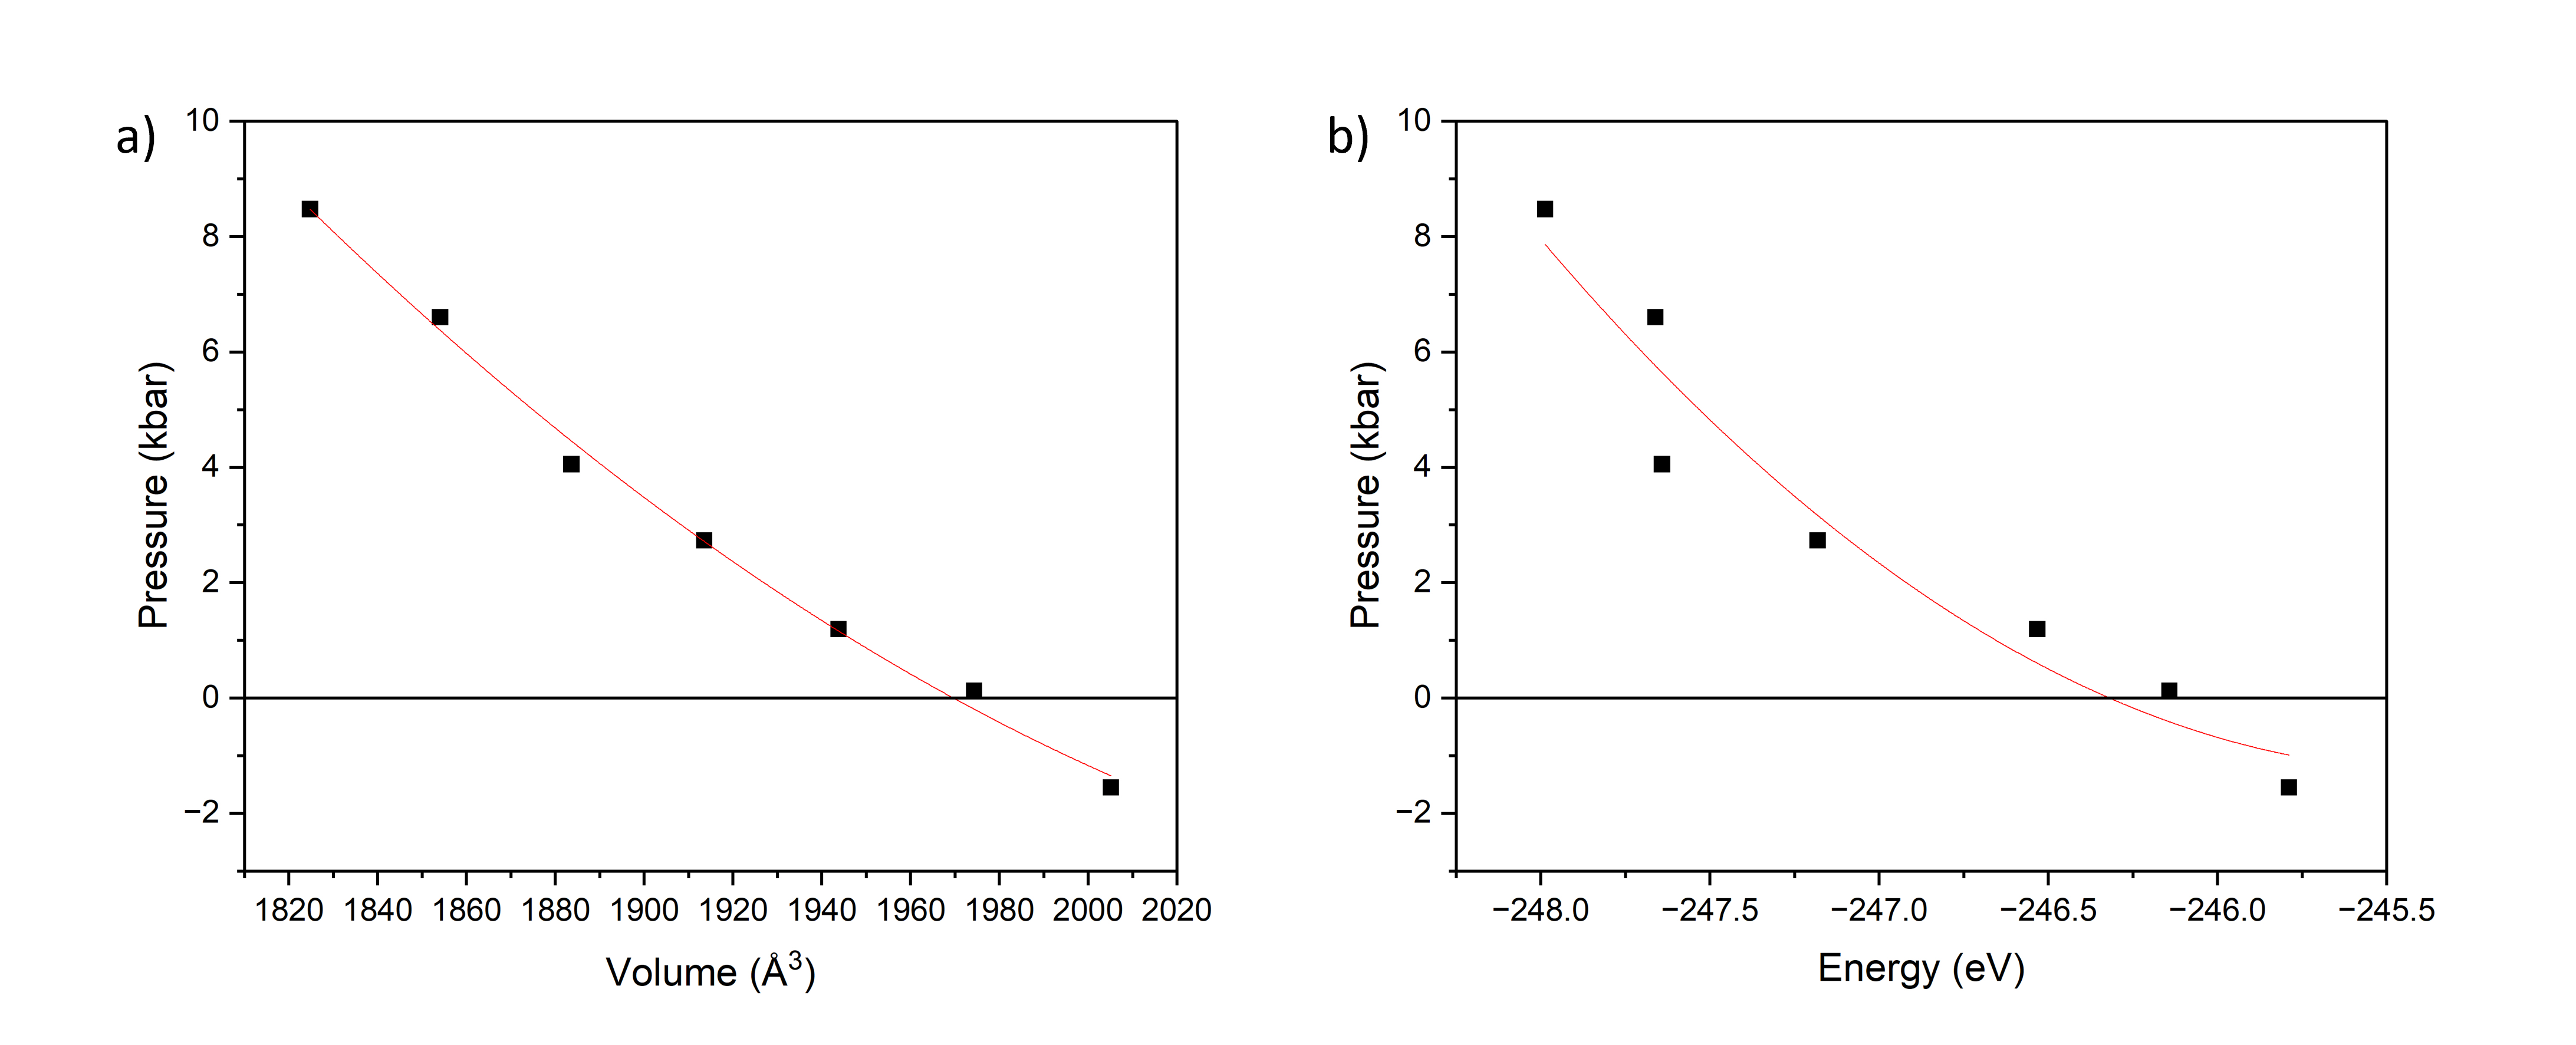
\includegraphics[width=\textwidth]{pv_pe_fixed.png}
\caption{An example of the a) pressure as a function of volume and b) pressure as a function of energy for the 16-42-42 mol\% composition at 1000 K.}
\label{fig:PV_PE}
\end{figure}
\FloatBarrier

In a similar manner used to determine the density, the heat capacity can also be found. The pressure as a function of potential energy, shown in \cref{fig:PV_PE}b, was determined by fitting a quadratic equation, allowing for the determination of the potential energy at which the pressure is zero. This zero-pressure potential energy is then added to the kinetic energy, and the total energy is plotted versus temperature. A linear function is fit to the data to obtain the total energy as a function of temperature. From this, the heat capacity can be determined:
\begin{equation}\label{eq:cp}
C_p=\lim_{\Delta T\to 0}\frac{\partial{E}}{\partial{T}}
\end{equation}
\noindent where $C_p$ is the heat capacity, T is the absolute temperature, and E is the total energy. It was verified that a linear function adequately represented the data, indicating a constant heat capacity over the temperature range investigated. 

The thermal expansion is determined by analyzing the zero-pressure volume as a function of temperature, treating the coefficient of thermal expansion ($\alpha$) as:

\begin{equation}\label{eq:cte}
\alpha = \frac{1}{V_0} \left(\frac{\partial{V}}{\partial{T}} \right)_p
\end{equation}

\noindent where $V_0$ is a reference volume at the lowest temperature explored for each composition. 

The enthalpy of mixing is determined from the potential energy of the mixed system and the three binary salts:
\begin{equation}
 \label{eq:Hmix}
 \Delta H^{mix} = \frac{E_{ABC}}{M_{ABC}} - \frac{x_A E_A}{M_A} - \frac{x_B E_B}{M_B} - \frac{x_C E_C}{M_C}
\end{equation}
where M$_i$ is the number of molecules in the system, E$_A$, E$_B$, and E$_C$ are the potential energies of the reference systems (LiF, NaF, and KF), E$_{ABC}$ is the potential energy of the ternary system, and $x_A$, $x_B$, and $x_C$ are the mole fraction of the respective reference salts in the mixture. This same equation can be applied to binary salt mixtures, reducing from four terms to three. While assumptions can be made to incorporate entropic effects to determine the free energy of mixing, such a step was not taken due to inherent assumptions required for ideal solution-type behavior. 

The binary and unary salt systems were equilibrated in a strictly NPT ensemble, easing some of the computational burden of exploring varied salt complexes, but limiting the ability to explore volume-dependent phenomena, such as the compressibility. There are no statistically significant differences in calculated thermodynamic quantities from the utilization of an NPT versus an NVT ensemble. 

\section{Results}

\subsection{Density and Thermal Expansion}

The density of each composition studied is displayed as a function of temperature in \cref{fig:densityVsTemp}. It should be noted that for all densities reported here, there is an approximate error of 0.05 g/cc. For all compositions, the density decreases with increasing temperature. This is in line with the inversely proportional relationship between density and temperature. The minimum density is observed for the pure LiF system, while the maximum density is observed for the NaF system. All of the densities fall within a range of approximately 0.25 g/cc, with the intermediate compositions having a much narrower range of only about 0.1 g/cc. Thus, the maximum variation for the ternary compositions is approximately 5\%. All data presented is also included in tabular form in the appendix. 

\begin{figure}[!h]
\centering
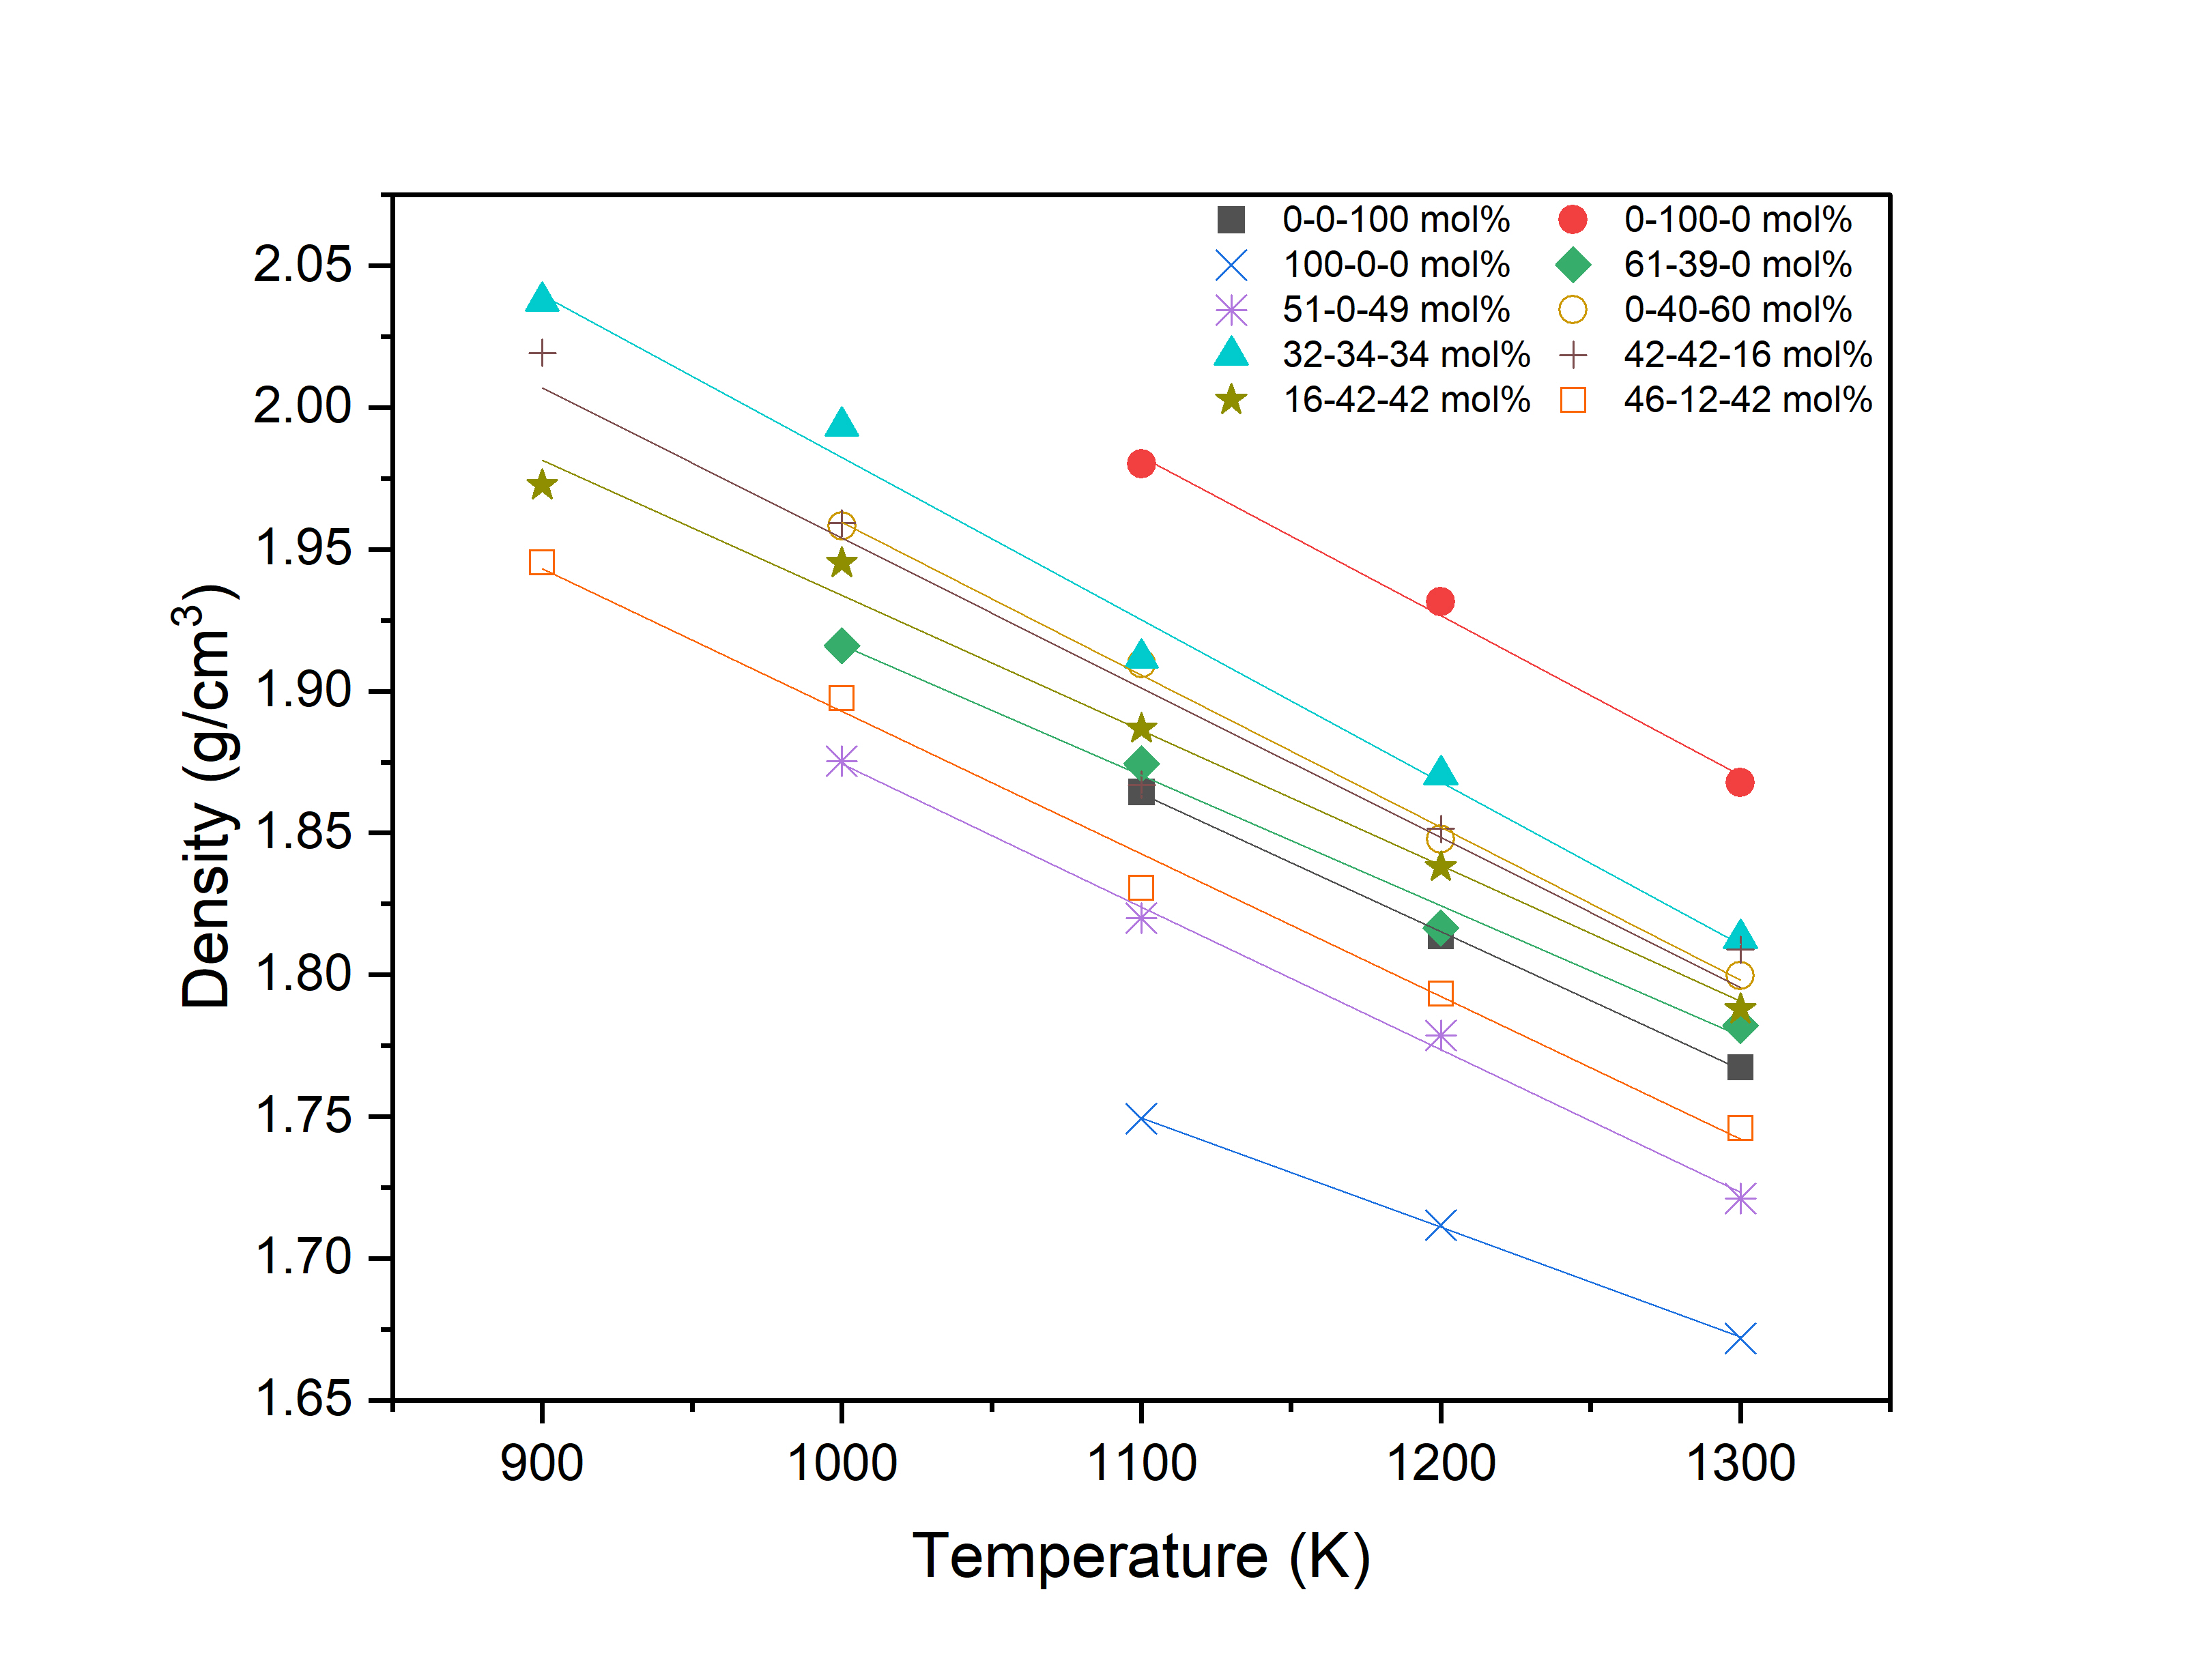
\includegraphics[width=.65\textwidth]{DensityVTemp_2.jpg}
\caption{The density (g/cm\textsuperscript{3}) versus temperature (K) of all compositions studied (LiF-NaF-KF mol\%).}
\label{fig:densityVsTemp}
\end{figure}

\noindent The density can be analyzed by composition, as in \cref{fig:density3comp}, where there is an overall decrease in the density as the percent of LiF increases. The opposite occurs in \cref{fig:density3comp}b, where the density increases as the percent of NaF increases. Looking at \cref{fig:density3comp}c, there appears to be little effect as the percent of KF changes. This seems to be reasonable, as the density of LiF is the lowest, the density of NaF is the highest, and the density of KF is at an intermediate value between the other two. It should be emphasized that in \cref{fig:density3comp}, ternary, binary, and unary salt densities are all included. 
\begin{figure}[!h]
    \centering
    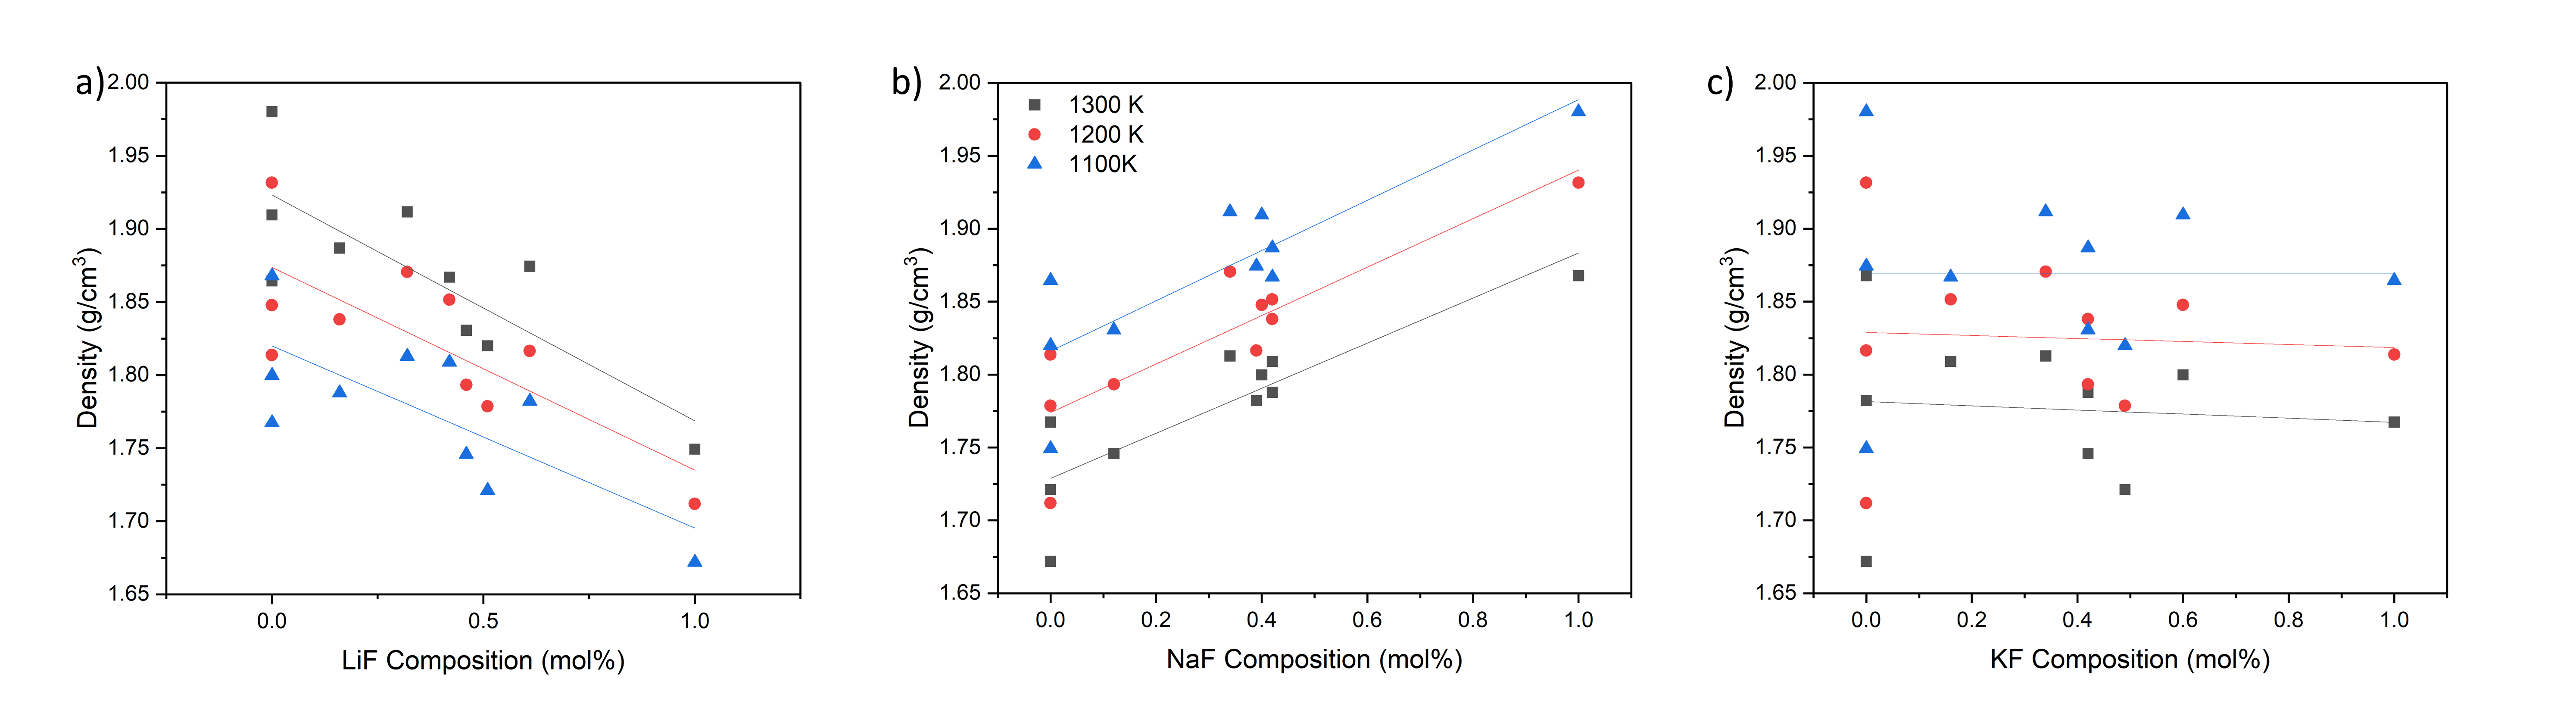
\includegraphics[width=\textwidth]{densityAll3_fixed.png}
    \caption{The density (g/cm\textsuperscript{3}) as a function of the composition of a) LiF (mol\%), b) NaF (mol\%), and c) KF (mol\%) for different FLiNaK salts.}
    \label{fig:density3comp}
\end{figure}
For the three temperatures at which all ten compositions were studied, ternary heatmaps, shown in \cref{fig:densityHeat}, were generated to better visualize the effects of the changing composition. While a limited number of compositions were utilized for the construction of the ternary density heat maps, they can clearly illustrate the dependence upon the composition. The composition of the mixture with respect to the LiF-NaF binary system is the primary determining factor for the density of the ternary, with the KF composition having nearly a negligible effect. It appears that density decreases more sharply as the composition nears LiF than the density decreases as the NaF composition increases, but additional data points at intermediate compositions would be required to verify these behaviors. For the four ternary phases, the eutectic is somewhat the outlier, possessing the least NaF and thus exhibiting the lowest density. The lower density of the eutectic composition compared to other ternary compositions may or may not be preferable. Regardless, these variations are somewhat minor. These conclusions hold across the temperature range studied. More complex density surfaces may be present but are not identifiable with the limited number of compositions studied here. 

\begin{figure}[h!]
    \centering
    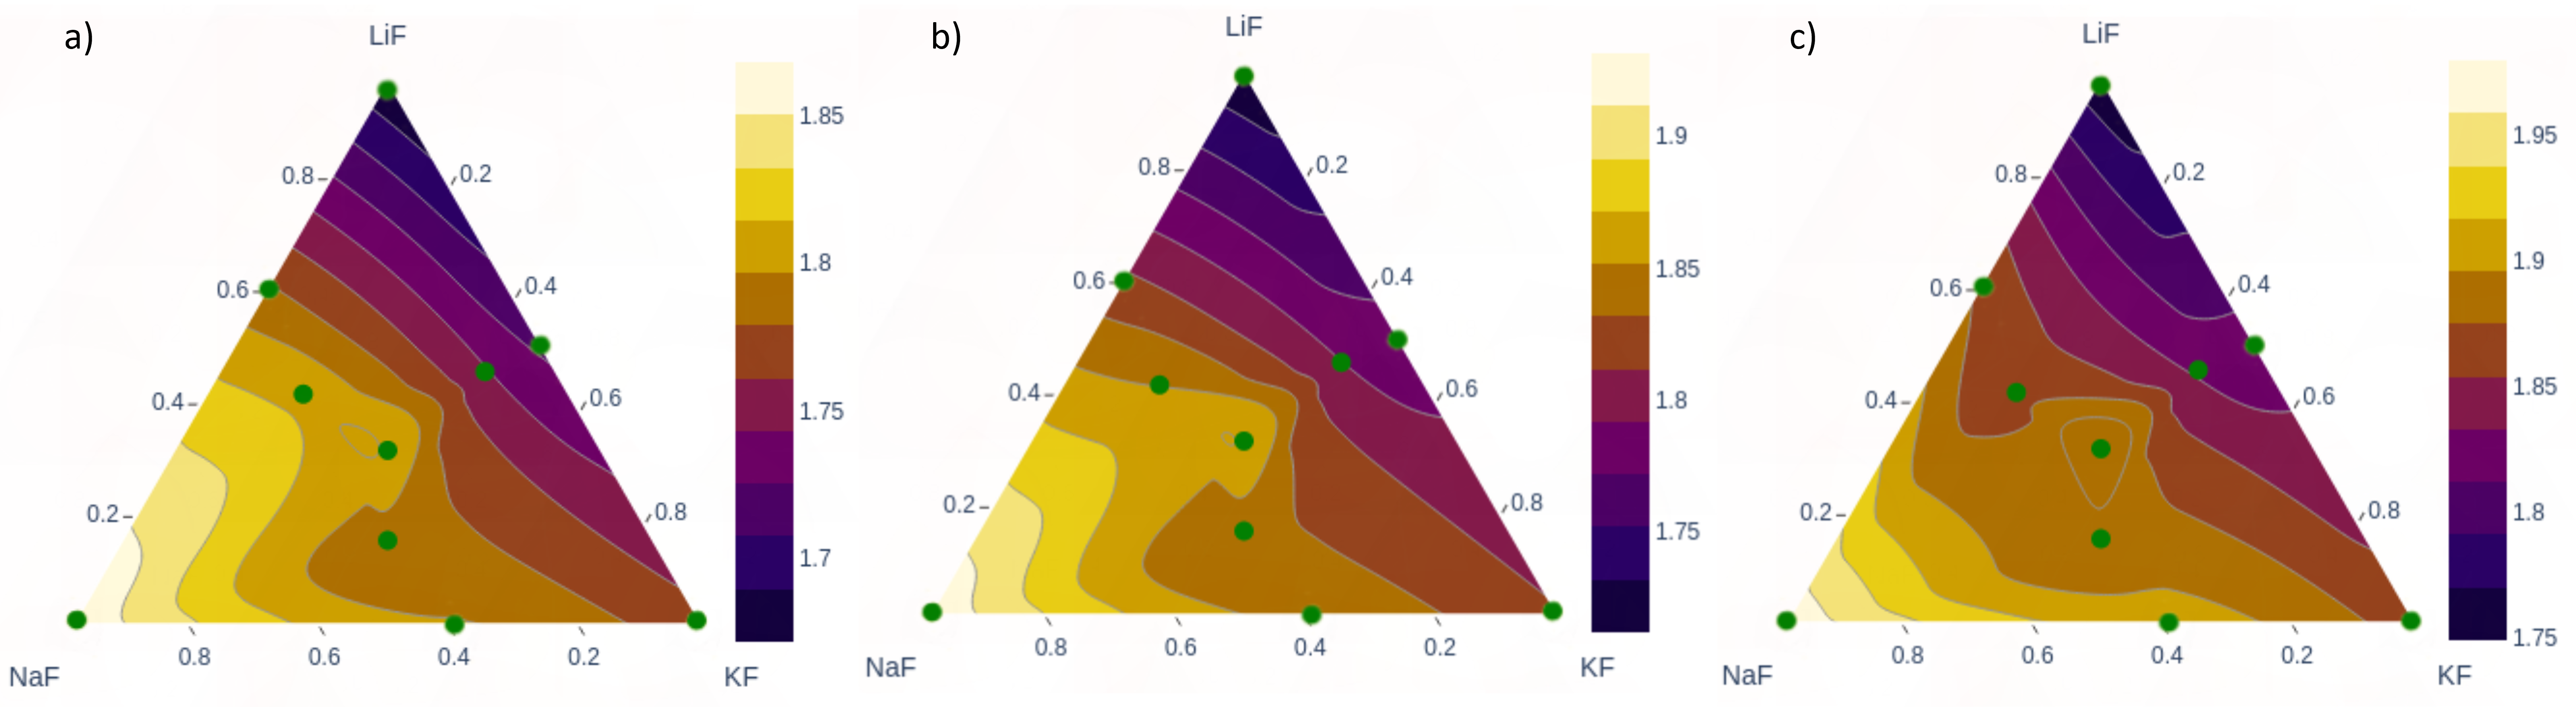
\includegraphics[width=0.95\textwidth]{densityTernary_withScatter.png}
    \caption{Ternary heatmap of the density (/cm\textsuperscript{3}) of FLiNaK at a) 1300 K, b) 1200 K, and c) 1100 K.}
    \label{fig:densityHeat}
\end{figure}

%\FloatBarrier

Experimental densities are available for comparison with the eutectic composition. When compared to experimental values from Janz \cite{Janz1981} (shown in \cref{fig:densityCompare}a), this work slightly underpredicts the density at all temperatures. The data deviates on average by 0.05 g/cc from Janz. %A more recent experimental study compared well with Janz but agreed more closely with our predictions for the density at 1300 K. 
For the individual salt endpoints (LiF, NaF, KF), the comparisons with experiments are shown in \cref{fig:densityCompare}b. There is a consistent, but minor, underprediction for the densities at all temperatures, but the change in the density with temperature shows good agreement, as the average deviation across all individual salts is 0.06 g/cc. As experimental measurements often report uncertainties on the order of 1-5\% \cite{JanzSaltProp}, there is general confidence in the magnitude and trends of the density with varying compositions. The error bars shown in \cref{fig:densityCompare} include a 2\% error from experiments, and a propagated computational error accounting for the scatter in each individual data point and the error from the quadratic fit, as illustrated in \cref{fig:PV_PE}. The error bars all predicted densities overlap with the error bars from experiments for all compositions and temperatures. 

\begin{figure}[!h]
\centering
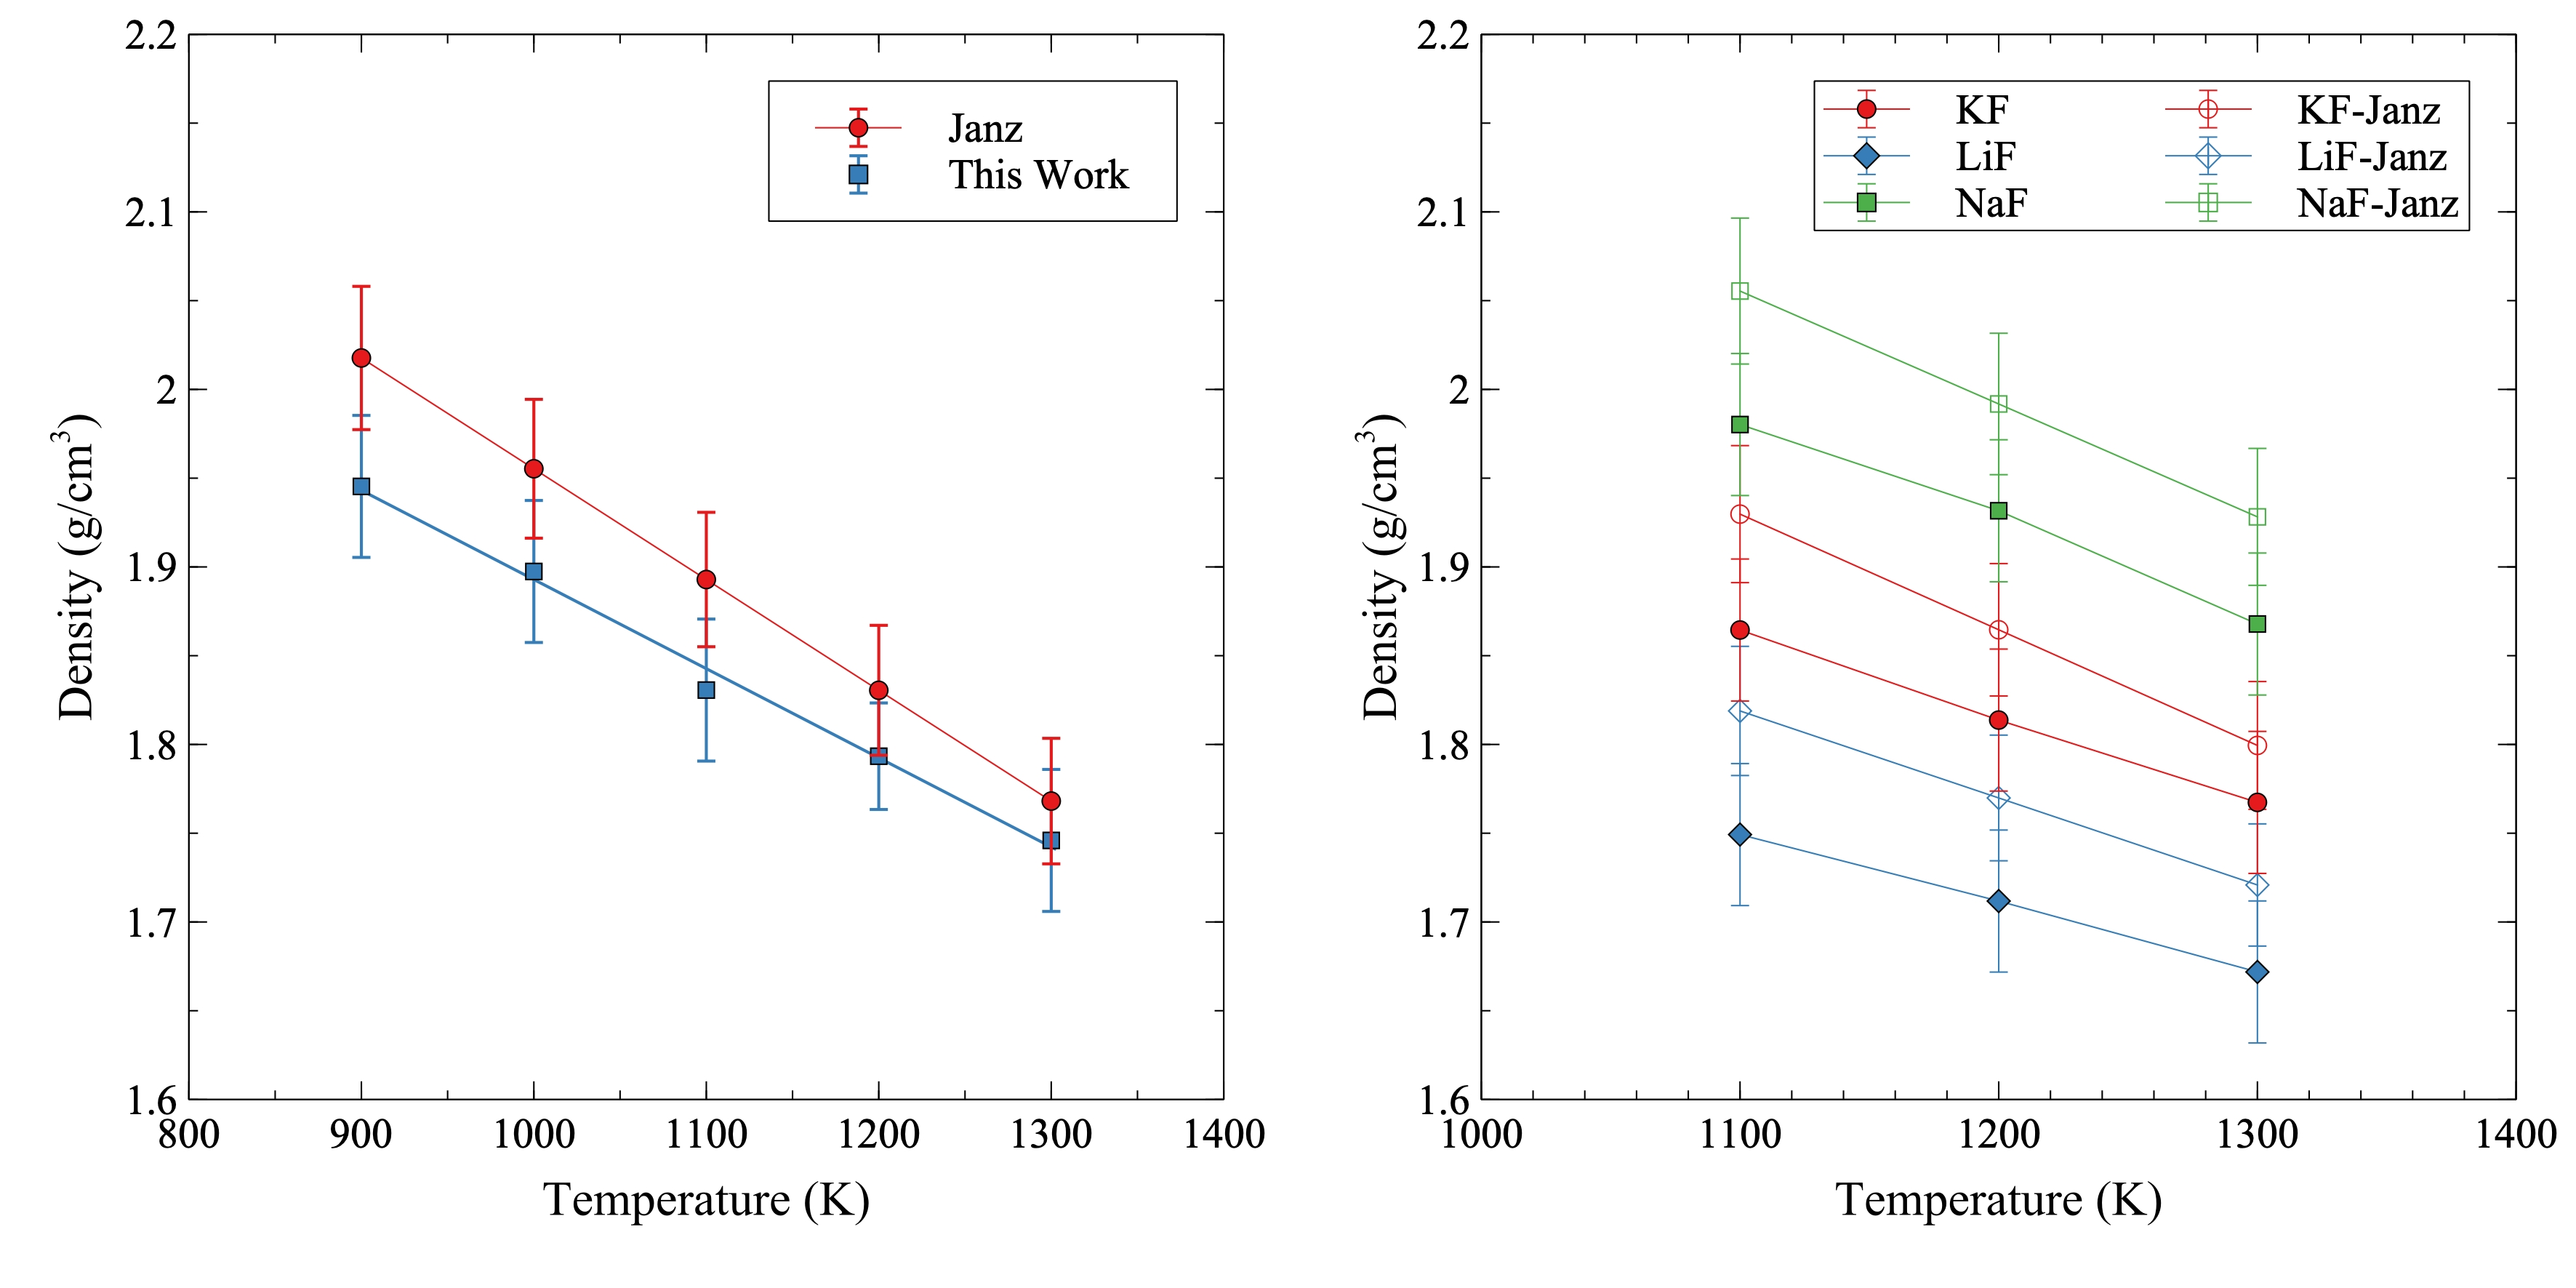
\includegraphics[width=0.95\textwidth]{fig5.jpg}
\caption{Comparison of density, g/cm\textsuperscript{3}, versus temperature, K, of a) the eutectic composition with literature\cite{Janz1981} and b) pure salts with literature\cite{JanzSaltProp}.}
\label{fig:densityCompare}
\end{figure}



The thermal expansion can be taken from the slope of the density in \cref{fig:densityVsTemp} with respect to temperature (\cref{eq:cte}). The thermal expansion coefficient is plotted versus composition in \cref{fig:therm3comp}. The trends of the thermal expansion with respect to composition are not as strong as those for density. The LiF concentration in \cref{fig:therm3comp}a has a negative impact on the coefficient of thermal expansion. However, as shown in \cref{fig:therm3comp}b and \cref{fig:therm3comp}c, there is not a statistically significant impact on the thermal expansion of varying compositions of NaF or KF. However, with increasing NaF and KF, there is a minor increase in the thermal expansion. The minimum thermal expansion of the four ternary compositions occurs at 16-42-42 mol \%, and the maximum occurs at 32-34-34 mol \%. When considering only the ternary compositions, the previously stated trends do not apply as there is no statistically significant relationship between the composition of the unary salts and thermal expansion.

\begin{figure}[!h]
    \centering
    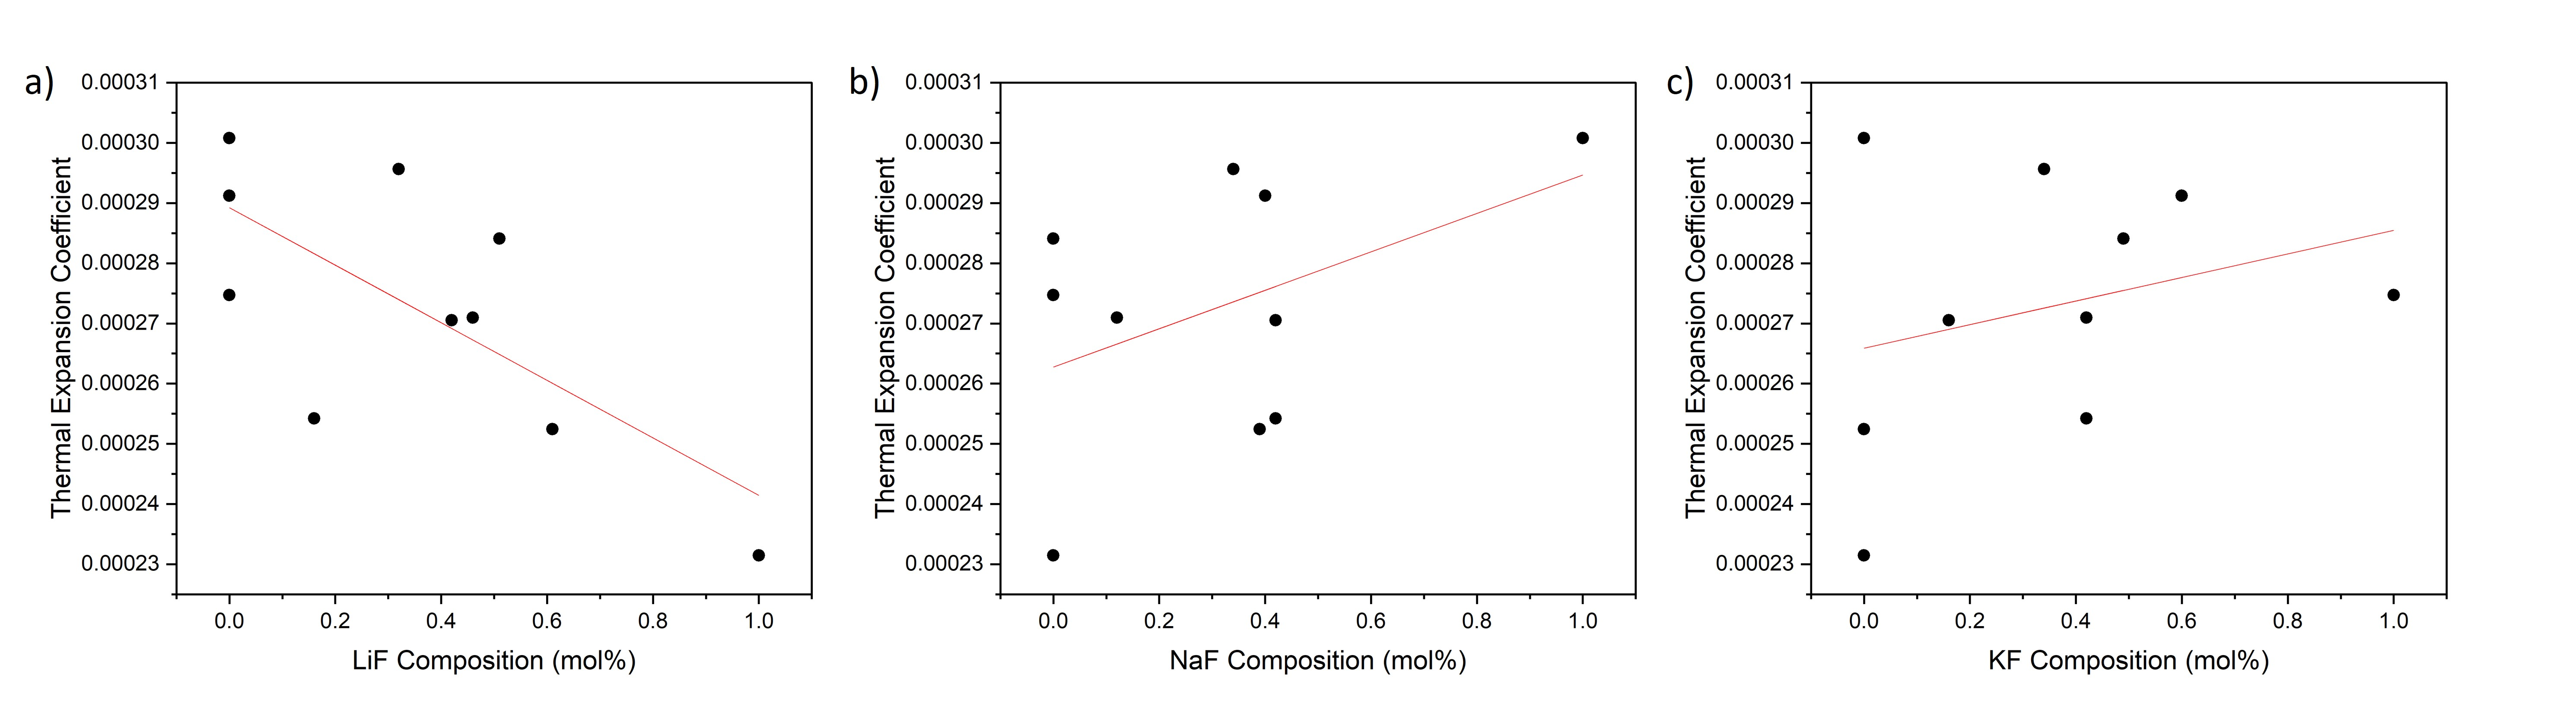
\includegraphics[width=0.95\textwidth]{thermalAll3_correctOrder.jpg}
    \caption{The thermal expansion coefficient versus the composition of a) LiF (mol\%), b) KF (mol\%), and c) NaF (mol\%) for different FLiNaK salts.}
    \label{fig:therm3comp}
\end{figure}

%\noindent The thermal expansion coefficient is displayed as a heatmap in \cref{fig:therm}. The heatmap shows that the thermal expansion is largest around the middle compositions, but there are no clear trends outside of that area. 

%\begin{figure}[!ht]
 %   \centering
  %  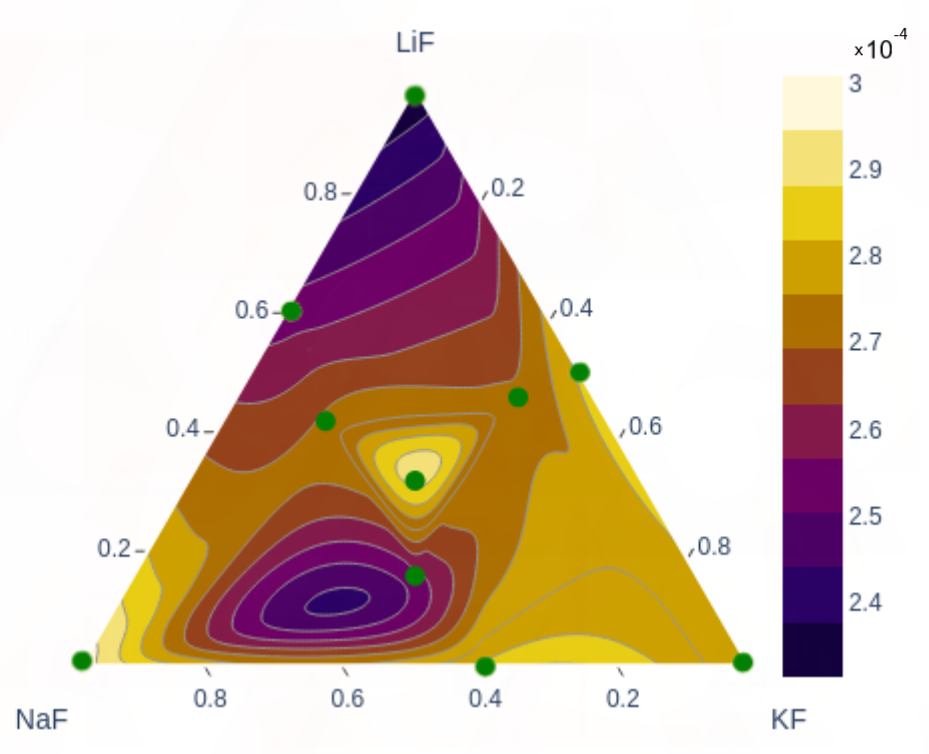
\includegraphics[width=.7\textwidth]{thermal_withScatterand104.png}
   % \caption{Ternary heatmap of the thermal expansion coefficient}
    %\label{fig:therm}
%\end{figure}
\FloatBarrier

\subsection{Bulk Modulus and Compressibility}

The bulk modulus and the compressibility are shown in \cref{fig:bulkCompress}. It should be emphasized that the compressibility is the inverse of the bulk modulus. Both are shown here for completeness. The degree of compressibility of a fluid has strong implications for its dynamics. As expected, the compressibility increases as the temperature increases. There is significant scatter in the data, which makes drawing specific conclusions regarding compositional dependence difficult, but generally, the eutectic composition has an intermediate value of the compressibility. The near equiatomic ternary salt has the lowest compressibility, and the low LiF content salt has the highest compressibility. Compared to two binary chloride salts (LiCl-KCl \cite{Duemmler2022} and NaCl-MgCl$_2$ \cite{Duemmler2022b}), the ternary compositions of FLiNaK display a lower value of the compressibility. Only ternary salts are included here as non-ternary compositions were analyzed in an NPT ensemble, which did not allow for the evaluation of the bulk modulus. 

\begin{figure}[!ht]
    \centering
    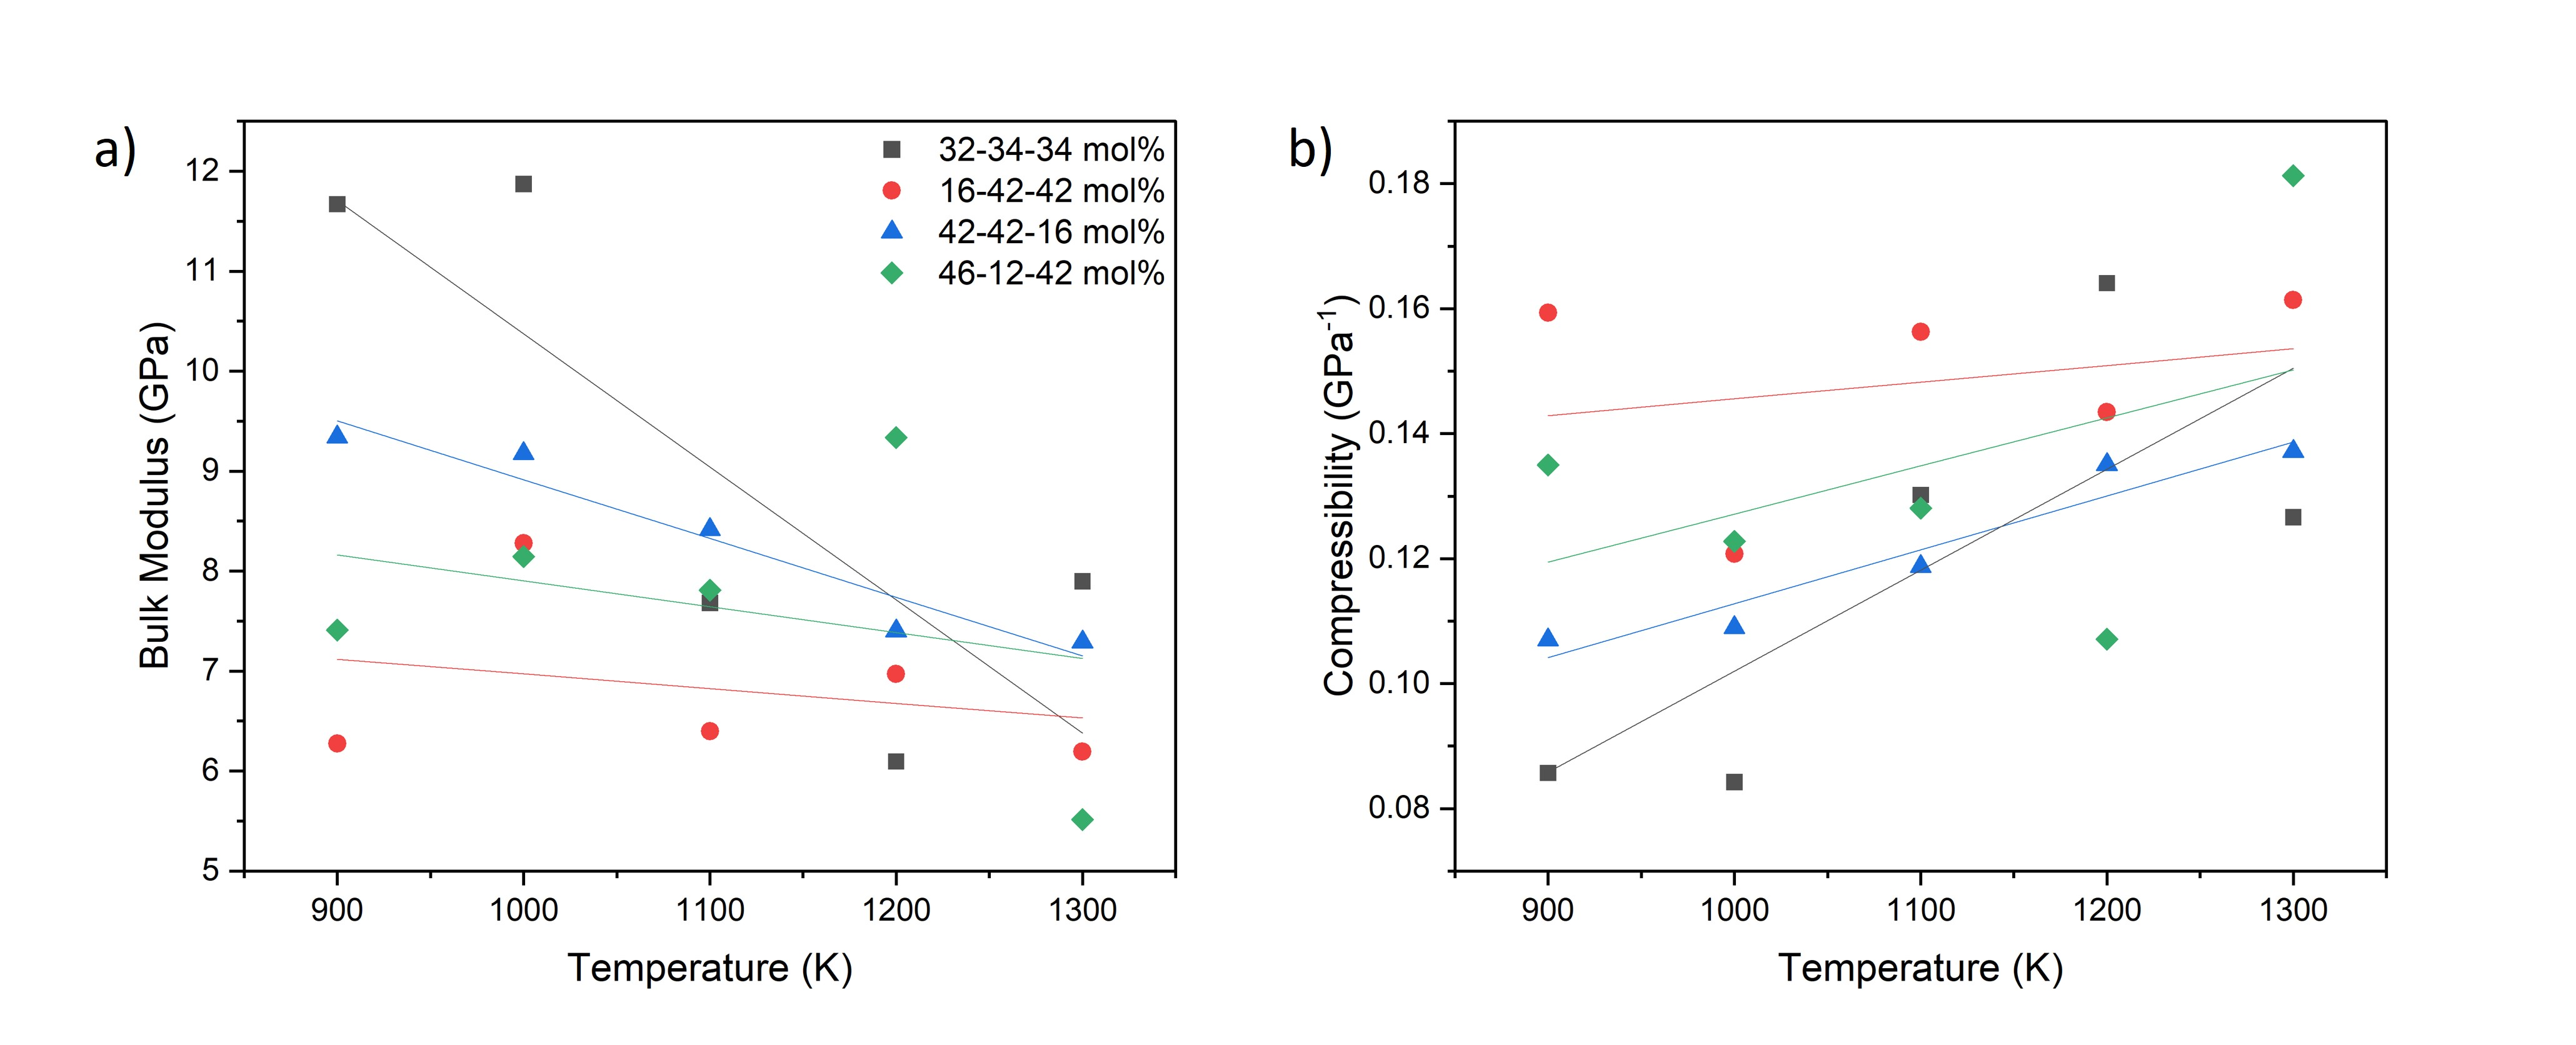
\includegraphics[width=\textwidth]{BulkCompress_2.jpg}
    \caption{a) Bulk modulus and b) compressibility of the four ternary compositions versus temperature}
    \label{fig:bulkCompress}
\end{figure}
\FloatBarrier

\subsection{Heat Capacity and Enthalpy of Mixing}

Heat capacity is a required parameter for thermal hydraulics models describing heat transport in molten salt systems\cite{freile2019}. The heat capacity for FLiNaK is best visualized as a ternary heatmap, shown in \cref{fig:Cp}. The heat capacity is greatest around the middle compositions and decreases as the system moves towards the three pure alkali-halide salt constituents. As stated, the exact contour locations may vary from their depiction here due to the limited number of ternary compositions, but the variance in the heat capacity with composition, in that a near equiatomic mixture has the highest heat capacity, is quite consistent. The total energy from AIMD simulations shows a linear dependence, thus the heat capacity is effectively constant over the investigated temperature range. Williams et al. report the heat capacity of the eutectic composition to be 77.9 J/mol-K at 973 K\cite{williams2006Cp}, which compares quite favorably to the calculated value of 67.6 J/mol-K from this work. Compared to the reported literature value, this work underpredicts the heat capacity by 13.2\%, but is neglecting the electronic contribution to the heat capacity, which, if included, would decrease the discrepancy. This is because the total heat capacity is a combination of the electron and phonon contributions to the heat capacity \cite{moore_uzr}, and including the electronic component will serve to increase the predicted value of the heat capacity. It should be noted that heat capacity measurements are notoriously difficult in molten salts, and often are in disagreement with one another \cite{robertson2022}. Generally, a higher heat capacity is preferable for thermal hydraulics applications, and thus this work points to a potential benefit of utilizing near-equiatomic compositions of FLiNaK. 

\begin{figure}[!ht]
    \centering
    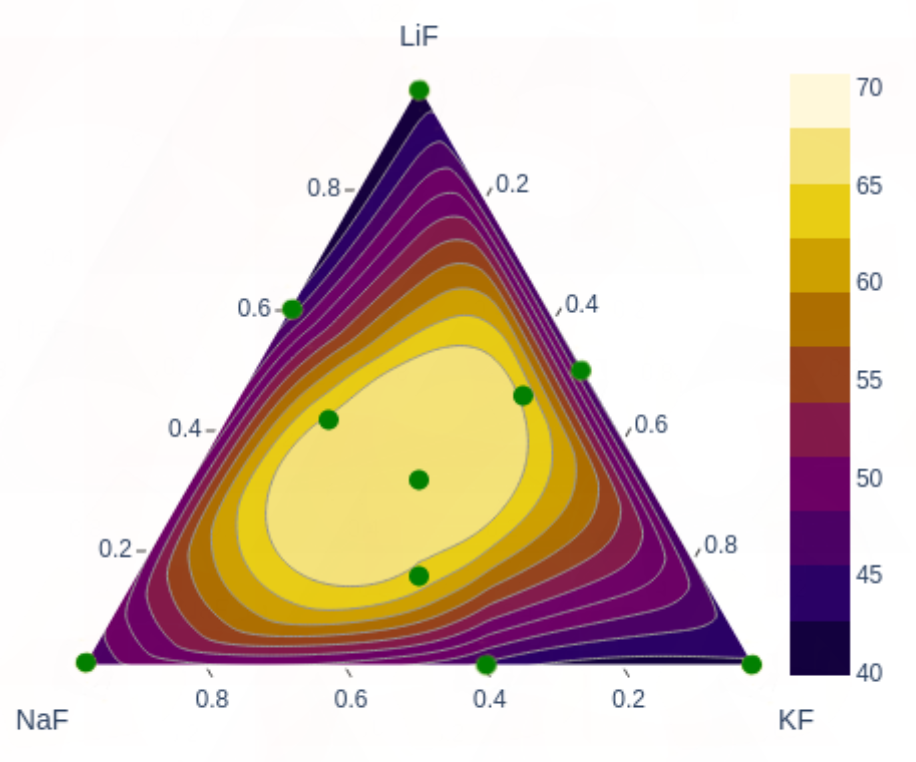
\includegraphics[width=.7\textwidth]{heatCapacity_withScatter.png}
    \caption{Ternary heatmap of the heat capacity of FLiNaK (J/mol-K).}
    \label{fig:Cp}
\end{figure}

The enthalpy of mixing is plotted against each of the pure alkali-halide salt constituents in \cref{fig:enth3comp}. Considering that this figure includes both ternary and binary compounds, the characteristic inverse hull shape is not present. However, intermediate compositions display the lowest enthalpy of mixing, with the near-equiatomic (32-34-34) composition exhibiting the global lowest energy. Including entropic effects to yield a free energy of formation was beyond the scope of this work, but it is anticipated that the near equiatomic composition would likely display the largest entropy, and thus the lowest free energy. Unfortunately, there is no experimental data for comparison. Additionally, prior computational investigations were typically restricted to the eutectic composition and did not explore the unary salt components, which prevented them from determining the enthalpy of formation. Experimental and additional computational studies are warranted to validate these results.

%Is there any experimental data for comparison?

%The expected parabolic shape is represented best in \cref{fig:enth3comp}a. When compared to each other, \cref{fig:enth3comp}b has the next closest shape to the expected one. \cref{fig:enth3comp}c does not resemble the expected parabola.

\begin{figure}[!ht]
    \centering
    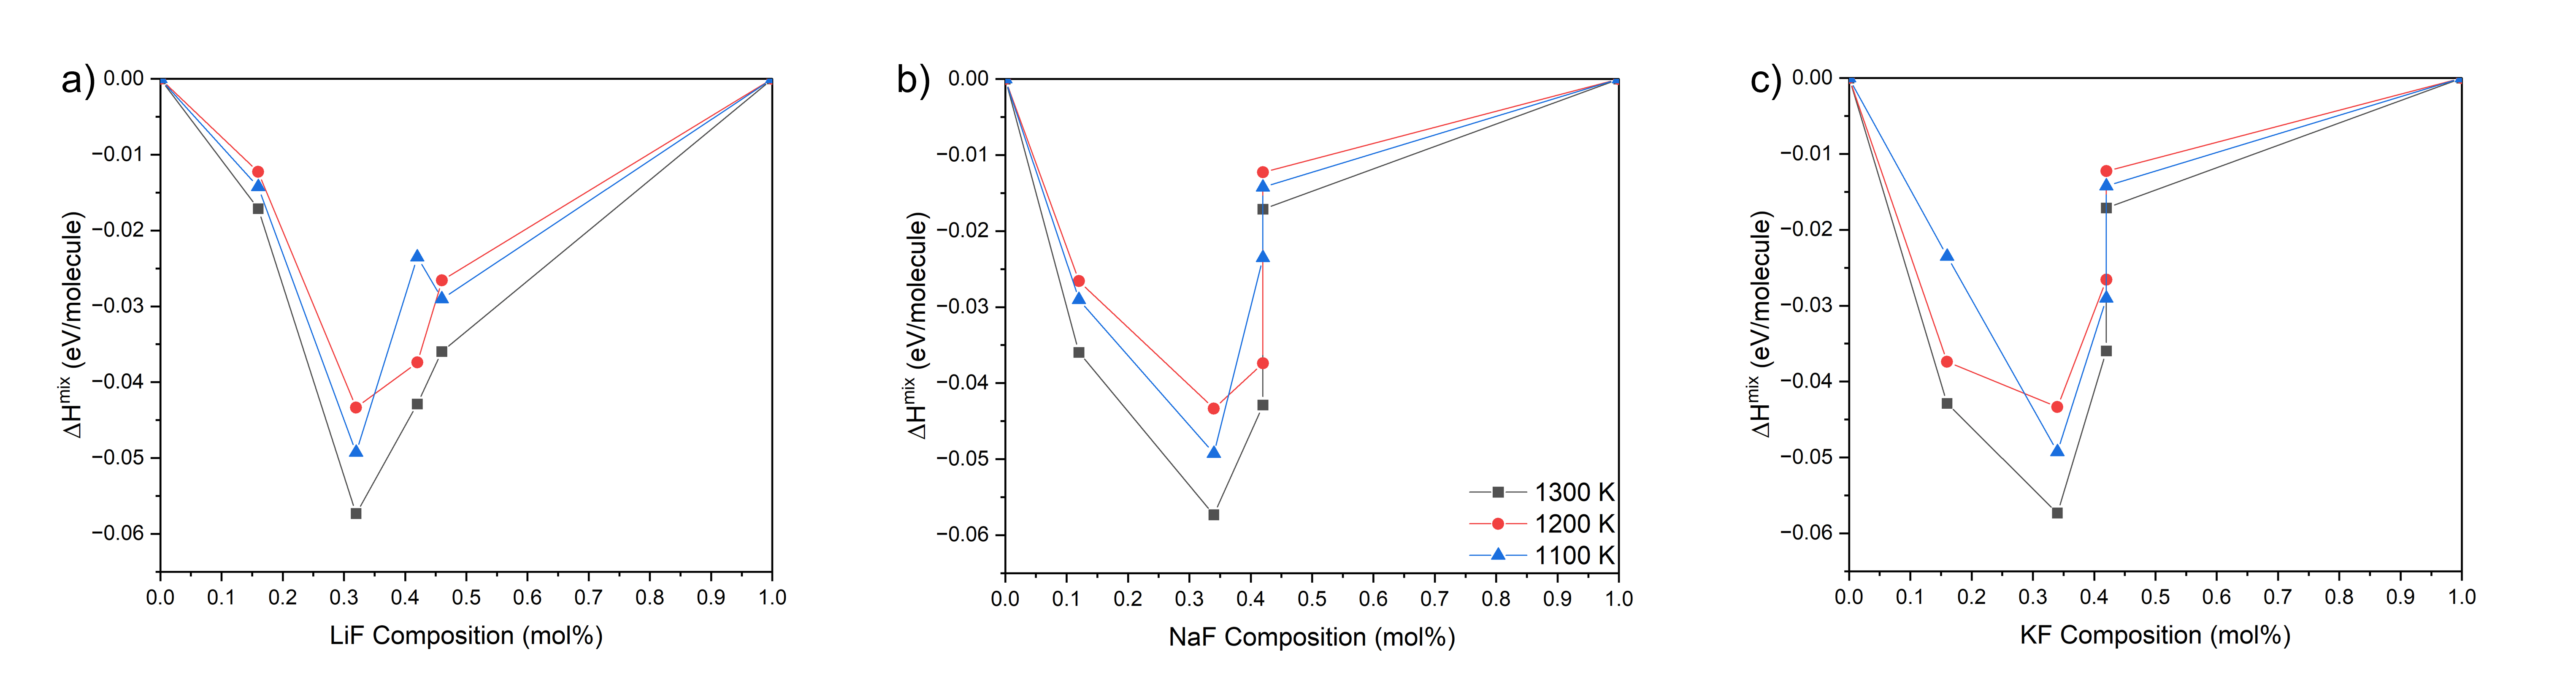
\includegraphics[width=\textwidth]{enthalpyMixAll3_fixed_part2.png}
    \caption{Graph of the enthalpy of mixing, eV/molecule, versus composition of a) LiF (mol\%), b) NaF (mol\%), and c) KF (mol\%).}
    \label{fig:enth3comp}
\end{figure}


\FloatBarrier


\subsection{Coordination Analysis}

The local atomic structure is analyzed by means of the radial pair distribution function (RDF). The RDF, or $g(r)$, measures the probability of finding a particle at distance $r$ given that there is a particle at position $r=0$. The peak of the RDF for each pair is the most probable location of the first-nearest-neighbor (1nn). The RDF for eutectic LiF-NaF-KF is shown in \cref{fig:rdf} at 900 K. Note that not all pair-wise interactions are shown in \cref{fig:rdf}, to aid in readability. Also, this RDF constitutes a time average over 3 ps of a given simulation at the zero-pressure volume at 900 K. The 1nn distance is then determined and compared to an x-ray diffraction study conducted at 793 K in \cref{table:cn}. Generally, the RDF compares very favorably to the experimental results, as well as a prior computational study \cite{Frandsen2020}. The most significant difference being for the F-F peak, which is overestimated by approximately 0.09 \AA. However, the experimental results assumed a Gaussian distribution for their analysis, which may induce small errors, and reported a mean square-root displacement of 0.41 {\AA}, indicating a broad peak, which is in accordance with these results and provides additional confidence in the accuracy of the simulations. The RDFs of the other ternary systems were analyzed to identify potential variations with somewhat minor compositional differences. The individual pair distances did not statistically change for the primary species, however, the F-F bond did show some variance depending upon the system, with the low Li concentration (16-42-42) displaying the longest F-F 1nn distance (3.33 \AA) and the eutectic displaying the shortest F-F bond 1nn distance (3.14 \AA) (\cref{tab:append_1nn}). There is not a clear correlation between F-F 1nn distance and density, which one might expect. However, there is a negative linear correlation (R$^2$=0.98) with the Li content, with greater Li content exhibiting shorter F-F 1nn distances. These minor structural variations would need to be confirmed via experiments and may provide insight into dynamical properties related to the distribution of F atoms in FLiNaK salts. 

\begin{figure}[!ht]
    \centering
    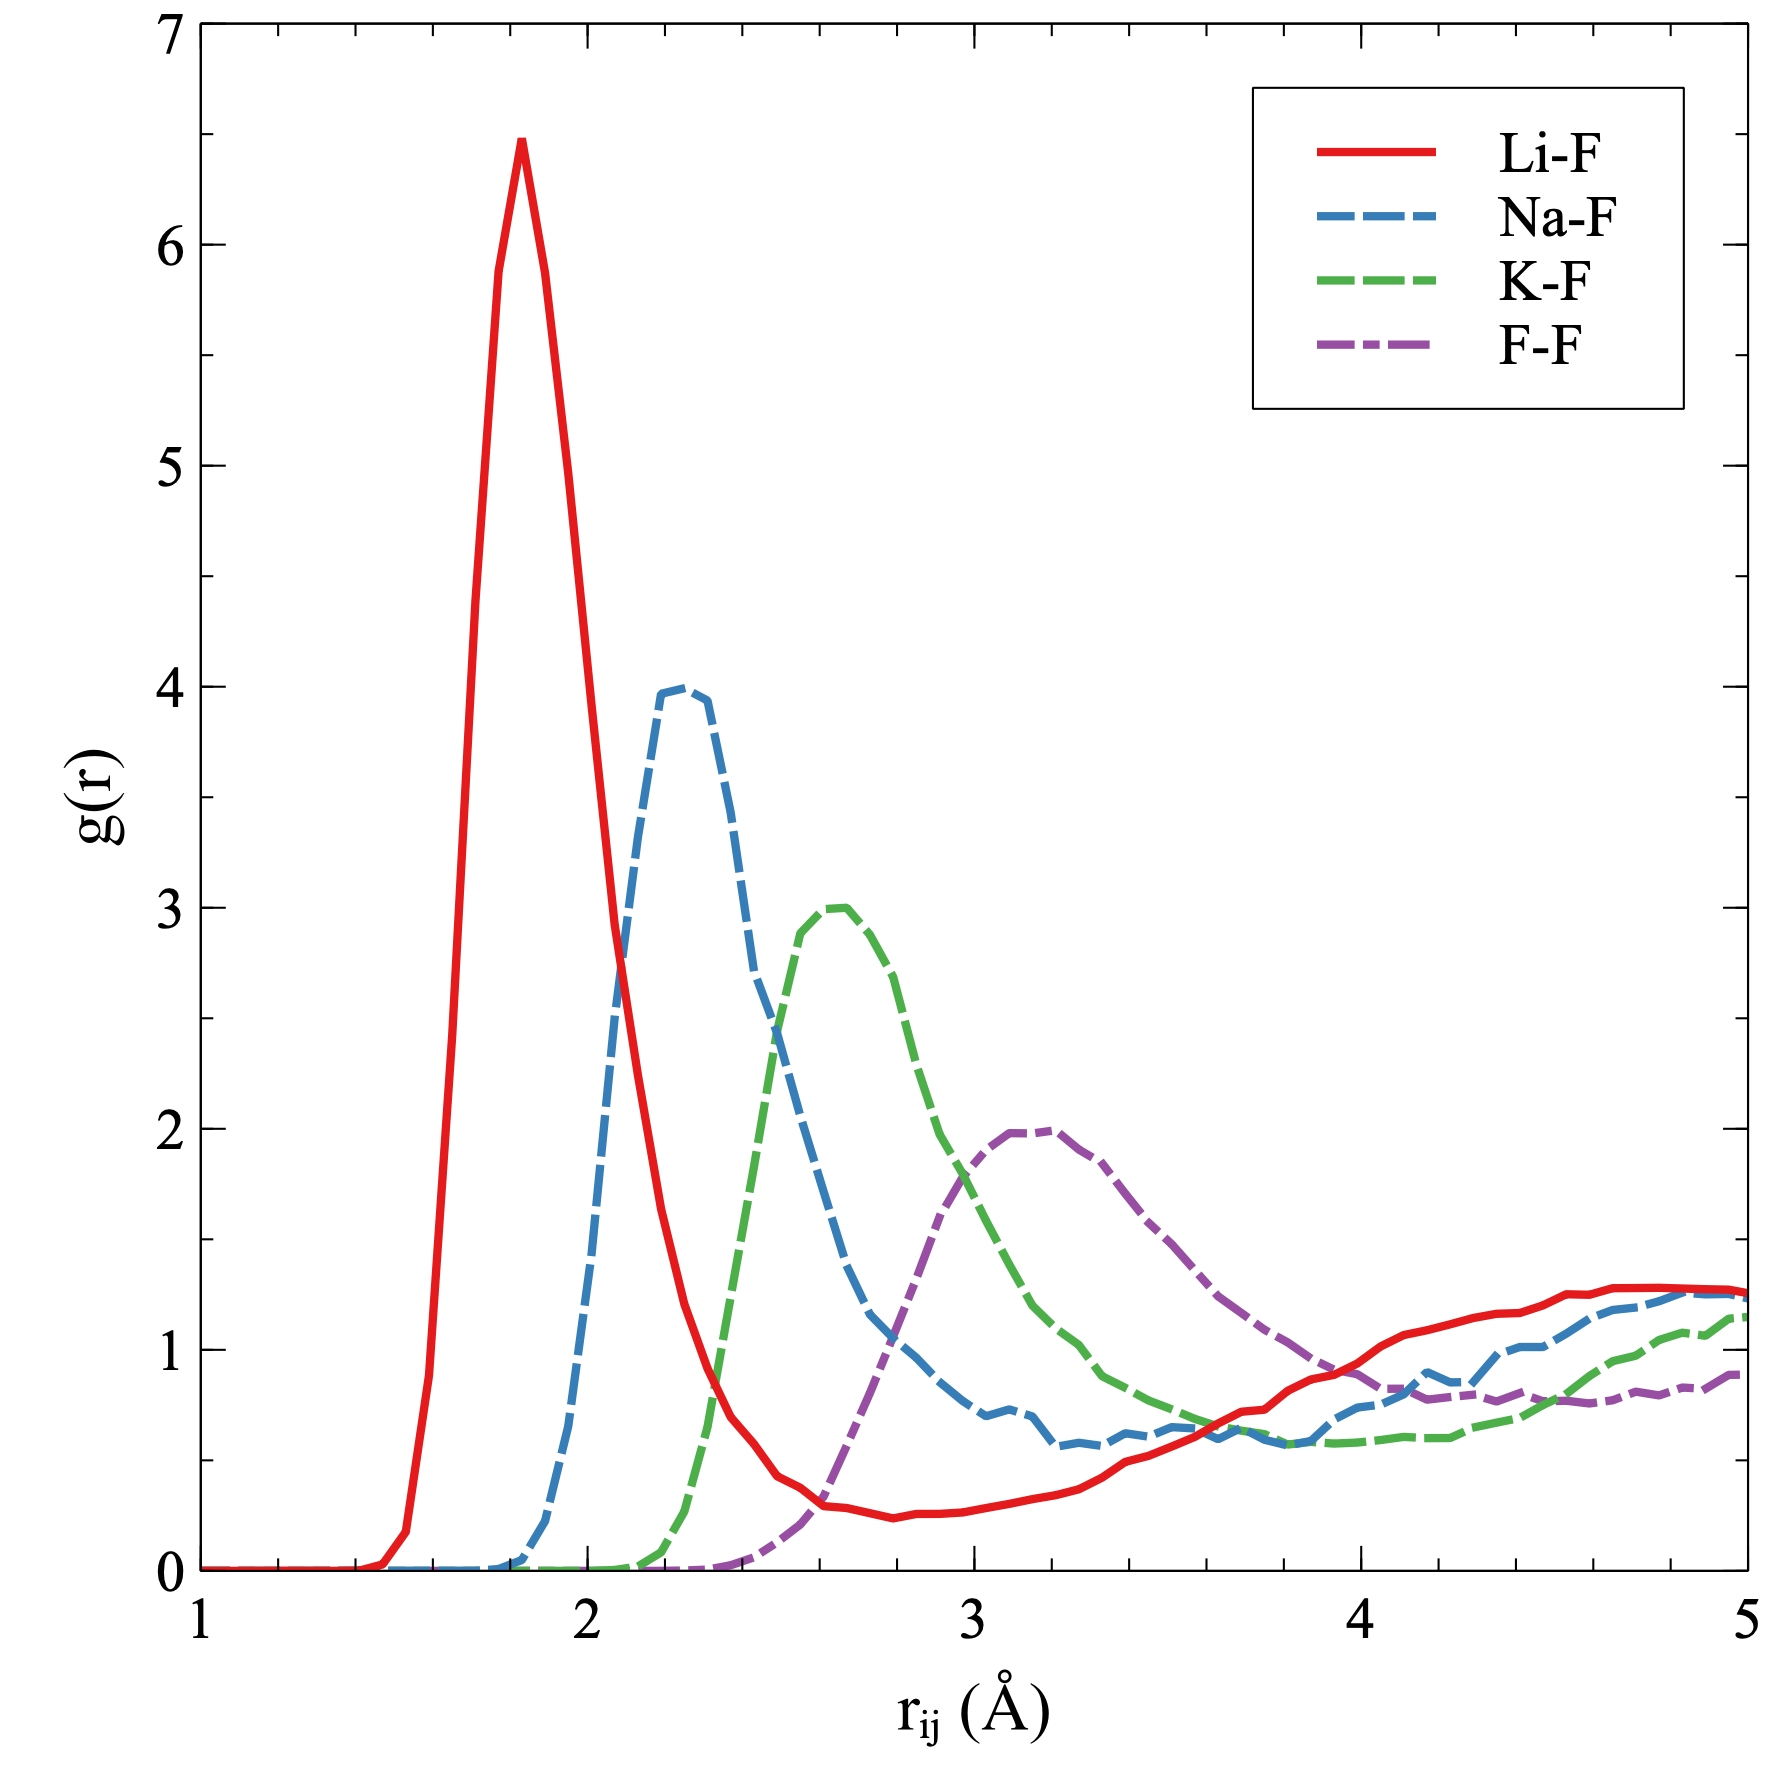
\includegraphics[width=0.5\textwidth]{final_rdf.jpg}
    \caption{Partial radial distribution functions for eutectic LiF-NaF-KF at 900 K.}
    \label{fig:rdf}
\end{figure}

\begin{table}[h!]
\centering
\caption{First nearest neighbor distances for eutectic LiF-NaF-KF at 900 K. Results are compared against experiment at 793 K \cite{igarashi1988}. }
\begin{tabular}{ccc}
\hline
Pair & r$_{ij}$(\AA)  & r$_{ij}$(\AA)\cite{igarashi1988}   \\
\hline
Li-F & 1.82 & 1.83 \\
Na-F & 2.23 & 2.18 \\
K-F & 2.64 & 2.59 \\
F-F & 3.14 & 3.05 \\
\hline
\end{tabular}
\label{table:cn}
\end{table} 

\FloatBarrier

\section{Conclusion}

To characterize the thermophysical properties of FLiNaK, a first principles computational investigation was performed for four ternary compositions, three binary eutectic compositions, and three pure alkali-halide salt constituents. The computational results of the density slightly underpredicted the experimental values at all temperatures for the eutectic and pure salt compositions. However, generally good agreement is observed. The density is positively correlated with the NaF concentration and negatively correlated with the LiF concentration. The thermal expansion was determined to decrease with increasing LiF concentration, but there was no statistically significant dependence on NaF or KF. The large scatter in the data for the bulk modulus and compressibility resulted in an inability to draw specific conclusions about compositional dependence, however, the compressibility increased with the temperature, as expected, and displays a magnitude lower than comparable chloride salts. The results for the heat capacity, like the density, underpredicted the literature value, but are likely within experimental uncertainties. In the enthalpy of mixing versus composition, the ternary compositions display the lowest formation energy, with the near equiatomic composition possessing the minimum. 


As the interest in molten salt reactors is renewed, there is a need for thermophysical properties of salt systems at varied compositions rather than just the eutectic composition. Currently, these properties are largely unknown, but can be elucidated through first principles methods. This work has shown that some thermophysical properties can exhibit significant differences with relatively minor compositional variance, indicating the potential for tailoring even well-known molten salt systems to target specific property behaviors. Further experimental work is necessary to validate the results presented in this manuscript, providing further confidence in the ability of first principles methods to explore the vast composition and temperature space relevant to molten salts in nuclear applications. 

%This is important because these properties are largely unknown at these compositions. To further this work, more investigation into various compositions not used here is needed. This work can also be expanded by using more temperatures. Both will give more insight into the important thermophysical properties of FLiNaK.


\section{Acknowledgements}
This work was supported through the NC State Nuclear Engineering Undergraduate Research Scholar Program with funding courtesy of the College of Engineering Enhancement Fee. This work is also supported through the INL Laboratory Directed Research and Development (LDRD) Program under DOE Idaho Operations Office Contract DE-AC07-05ID14517. This research made use of the resources of the High-Performance Computing Center at Idaho National Laboratory, which is supported by the Office of Nuclear Energy of the U.S. Department of Energy and the Nuclear Science User Facilities. 

\appendix
\setcounter{table}{0}
\section{}

\begin{table}[h]
\centering
\caption{The density (g/cm$^{3}$) of LiF-NaF-KF at different temperatures. }
\begin{tabular}{|c|ccccc|}
\hline
Composition (LiF-NaF-KF) & 900 K &  1000 K  & 1100 K  & 1200 K & 1300 K    \\
\hline
eutectic 46-12-42 & 1.95 & 1.90 & 1.83 & 1.79 & 1.75 \\
16-42-42 & 1.97 & 1.95 & 1.89 & 1.84 & 1.79       \\
32-34-34 & 2.04 & 1.99 & 1.91 & 1.87 & 1.81       \\
42-42-16 & 2.02 & 1.96 & 1.87 & 1.85 & 1.81       \\
0-40-60  & - & 1.96 & 1.91 & 1.85 & 1.80       \\
51-0-49  & - & 1.88 & 1.82 & 1.78 & 1.72       \\
61-39-0  & - & 1.92 & 1.87 & 1.82 & 1.78       \\
100-0-0  & - & - & 1.75 & 1.71 & 1.67       \\
0-100-0  & - & - & 1.98 & 1.93 & 1.87       \\
0-0-100  & - & - & 1.86 & 1.81 & 1.77       \\
\hline
\end{tabular}
\label{tab:append_dens}
\end{table}
\FloatBarrier

\begin{table}[h]
\centering
\caption{The coefficient of thermal expansion ($\alpha$), compressibility ($\beta$ at 1100 K), heat capacity ($C_P$), and enthalpy of mixing ($\Delta H_{mix}$ at 1300 K) of LiF-NaF-KF.}
\begin{tabular}{|c|c|c|c|c|}
\hline
Composition (LiF-NaF-KF) & $\alpha \times10^{-4}$ & $\beta$ (GPa$^{-1}$) & $C_P$ (J/mol-K) & $\Delta H_{mix} (eV/molecule)$ \\
\hline
eutectic 46-12-42 & 2.88 & 0.128 & 67.6 & -0.027\\
16-42-42 & 2.66 & 0.121 & 66.8 & -0.017 \\
32-34-34 & 3.15 & 0.130 & 70.7  & -0.057 \\
42-42-16 & 2.93 & 0.119 & 68.3 & -0.043  \\
0-40-60  & 2.91 & - &  43.1 & -0.007   \\
51-0-49  & 2.84 & - &  43.0 & -0.043  \\
61-39-0  & 2.52 & - &  42.0 & -0.028 \\
100-0-0  & 2.31 & - &  39.9 & -  \\
0-100-0  & 3.01 & - &  44.4 & - \\
0-0-100  & 2.75 & - &  41.9 & -  \\
\hline
\end{tabular}
\label{tab:append_prop}
\end{table}
\FloatBarrier


\begin{table}[h]
\centering
\caption{The first-nearest-neighbor distances of the ternary LiF-NaF-KF salts at 900K.}
\begin{tabular}{|c|c|}
\hline
Composition (LiF-NaF-KF) & F-F 1nn distance (\AA) \\
\hline
eutectic 46-12-42 & 3.14 \\
16-42-42 & 3.33 \\
32-34-34 & 3.21 \\
42-42-16 & 3.15  \\
\hline
\end{tabular}
\label{tab:append_1nn}
\end{table}

\FloatBarrier

\bibliographystyle{elsarticle-num} 
\bibliography{cas-refs}


\end{document}

